\chapter{Introduction}
\section{Objectifs et choix}
Dans le cadre de l'apprentissage des fonctionnements des interfaces systèmes/réseaux et des sockets, nous avons choisi de réaliser un serveur FTP. Le programme sera réalisé en C. Les manipulations des sockets se font donc au plus bas niveau. Cette absence d'abstraction nous a obligé à comprendre les différents comportements des sockets. Le choix de réaliser un serveur FTP a été conditionné par les raisons suivantes 
\begin{itemize}
	\item
		L'opportunité de progresser dans la compréhension du fonctionnement des application clients/serveurs. En effet ce protocole est illustation simple de ce type de fonctionnement (cf 1.2).
	\item{}
		La relative simplicité et l'absence d'interface graphique pour laisser tout le temps de travail à la manipulations d'outils réseaux.
	\item{}
		Un protocole dédié au transferts de fichier est idéal pour se être confronté à un maximum de problèmes de type réseau. 		
\end{itemize}

\section{Rappels sur le protocole FTP}
Le protocole FTP à une architecture client/serveur spécifique dont les grandes lignes sont illustrées ci-après : 

\begin{figure}[!h] 
\begin{center}
  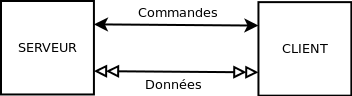
\includegraphics{cs.png}
\end{center}
\caption{Liens Serveur/Client}
\end{figure} 
Deux liens de communication relie un client au serveur. Un pour un dialogue (commandes clients, informations serveurs ...), l'autre pour le transit des données.
On rappel que les objectifs du serveur FTP sont les suivants : 

\begin{itemize}
    \item{}
	 permettre un partage de fichiers entre machines distantes.
    \item{}
	 permettre une indépendance aux systèmes de fichiers des machines clientes et serveur.
    \item{}
	permettre de transférer des données de manière efficace.
\end{itemize}


Le but de ce projet est de réaliser une telle architecture de manière à ce que plusieurs clients puissent se connecter en même temps.
\begin{figure}[!h] 
\begin{center}
  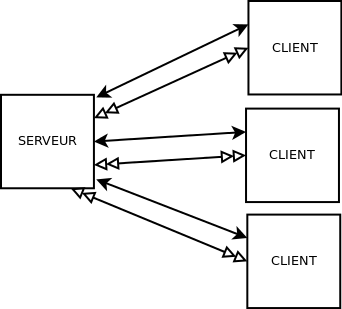
\includegraphics{cs2.png}
\end{center}
\end{figure} 
